\section{Experimental data}
The following data was obtained by experimentally running the specified test case and collecting the necessary data.
Data processing and graphic generation has been performed using Matlab \cite{sw:matlab}.

All presented graphs include the set-point values curve as well as the feedback values curve.
After the following subsections, a table is shown that presents the following measured characteristics of the step-response of the controlled variable for the corresponding test case: rise-time, settling-time, overshoot, peak value and peak time.

Because our speed calculation algorithm provides values with reduced precision, the computed speed value continuously jumps between step values due to the nature of the algorithm (see \autoref{speed-algorithm}).
This is the reason why the feedback curve shown in the following figures oscillates slightly while the set-point value remains constant.
As such, we had to adjust the setting-time margin from the default 2\% to 5\%.

\clearpage

\subsection*{Local control mode, 5ms network cycle time}
\begin{figure}[H]
	\centering
	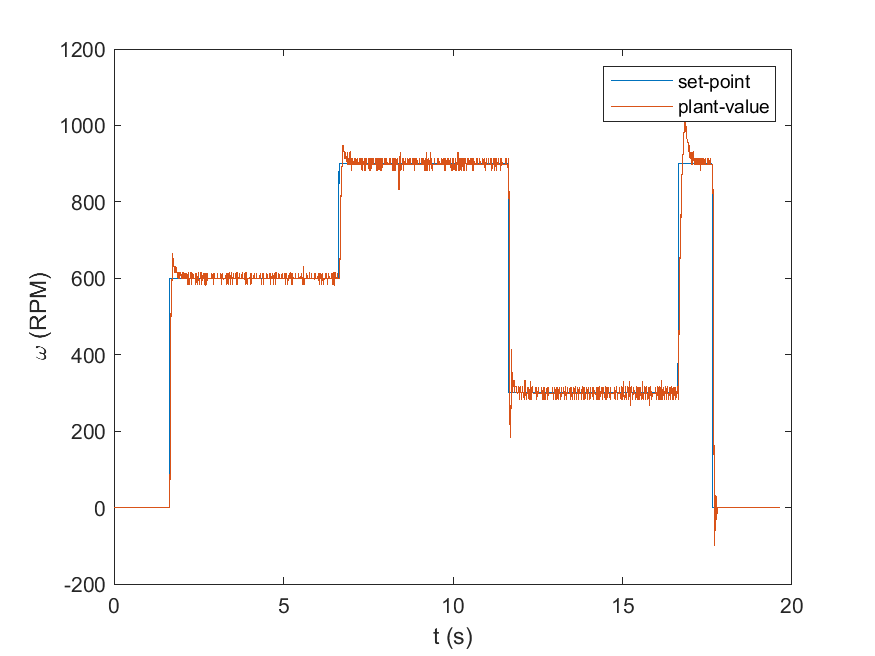
\includegraphics[width=0.8\linewidth]{local-5ms.png}
	\caption{Set-point and feedback value curves for local control with 5ms network cycle time}
	\label{fig:local-5ms}
\end{figure}

\subsection*{Remote control mode, 5ms network cycle time}
\begin{figure}[H]
	\centering
	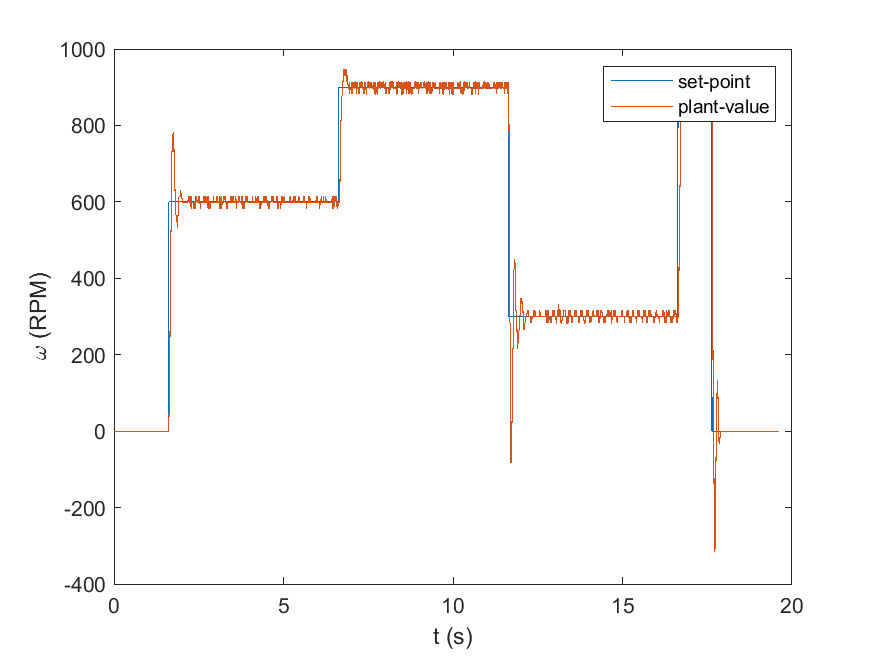
\includegraphics[width=0.8\linewidth]{remote-5ms.png}
	\caption{Set-point and feedback value curves for remote control with 5ms network cycle time}
	\label{fig:remote-5ms}
\end{figure}

\subsection*{Local control mode, 10ms network cycle time}
\begin{figure}[H]
	\centering
	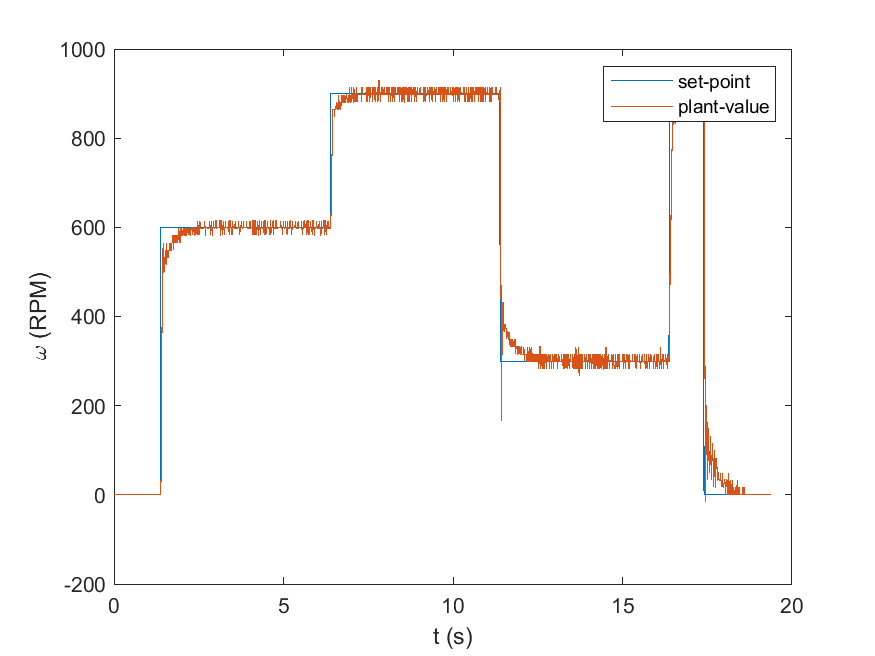
\includegraphics[width=0.8\linewidth]{local-10ms.png}
	\caption{Set-point and feedback value curves for local control with 10ms network cycle time}
	\label{fig:local-10ms}
\end{figure}

\subsection*{Remote control mode, 10ms network cycle time}
\begin{figure}[H]
	\centering
	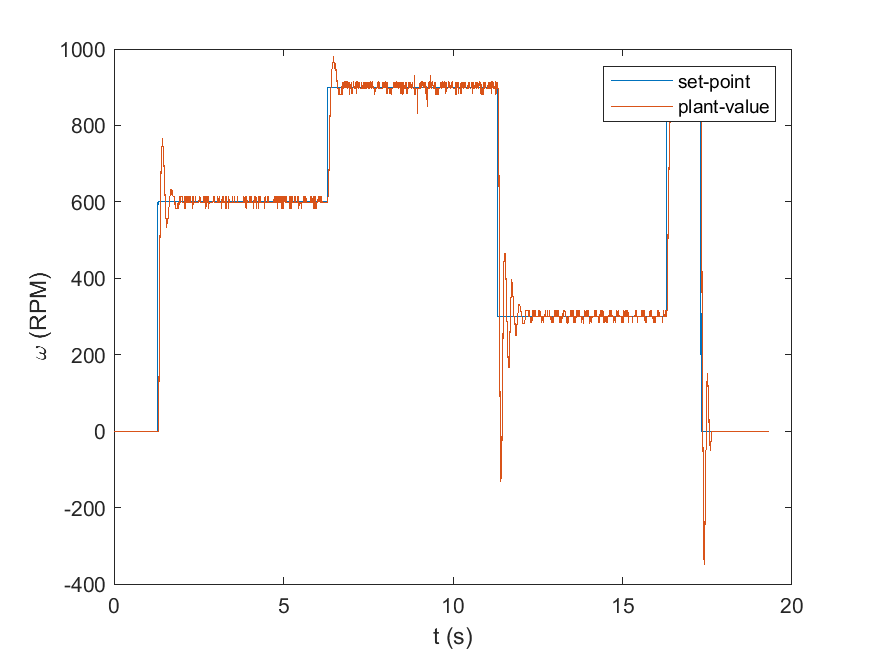
\includegraphics[width=0.8\linewidth]{remote-10ms.png}
	\caption{Set-point and feedback value curves for remote control with 10ms network cycle time}
	\label{fig:remote-10ms}
\end{figure}

\subsection*{Local control mode, 20ms network cycle time}
\begin{figure}[H]
	\centering
	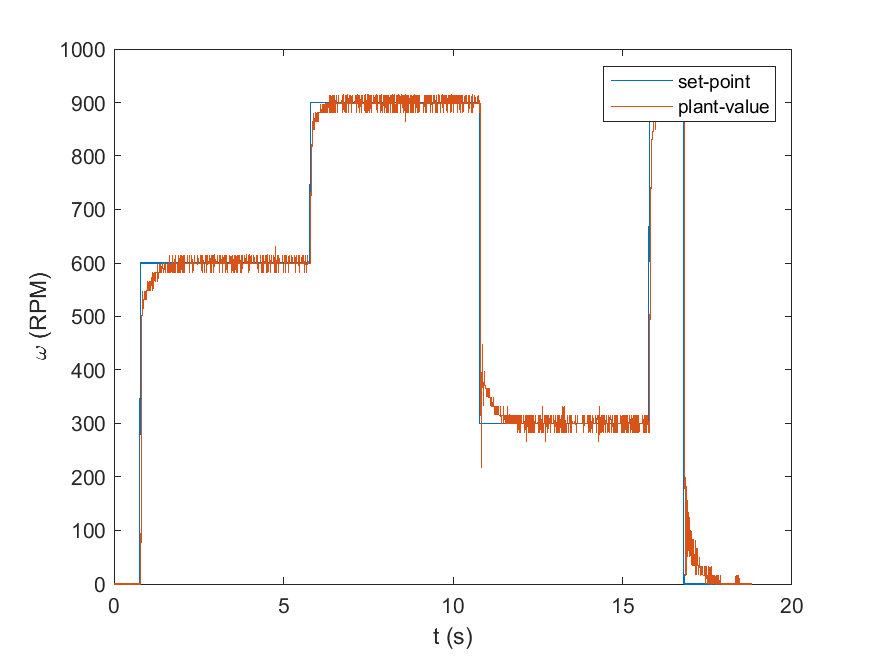
\includegraphics[width=0.8\linewidth]{local-20ms.png}
	\caption{Set-point and feedback value curves for local control with 20ms network cycle time}
	\label{fig:local-20ms}
\end{figure}

\subsection*{Remote control mode, 20ms network cycle time}
\begin{figure}[H]
	\centering
	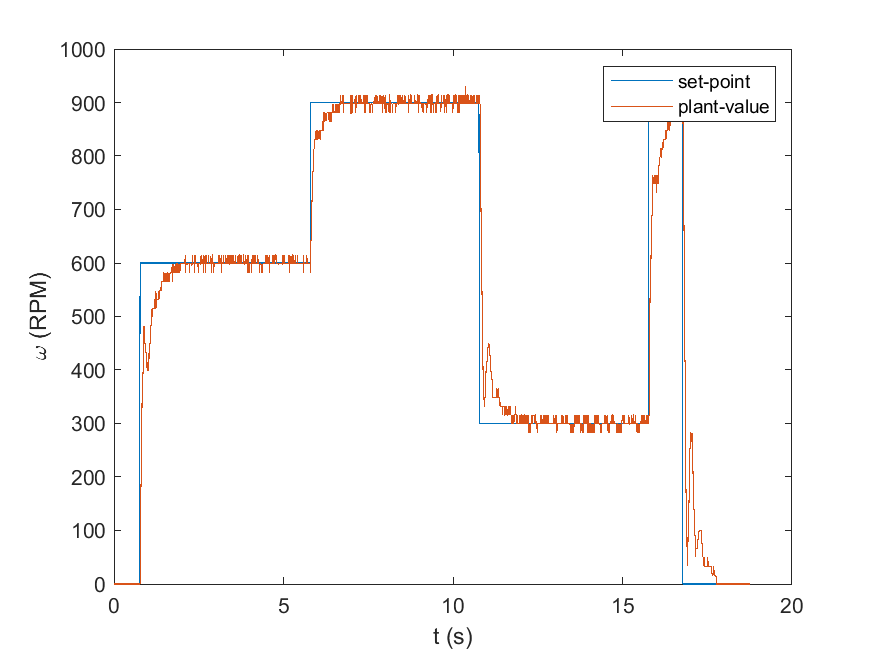
\includegraphics[width=0.8\linewidth]{remote-20ms.png}
	\caption{Set-point and feedback value curves for remote control with 20ms network cycle time}
	\label{fig:remote-20ms}
\end{figure}

\subsection{Data analysis}

\autoref{tab:step-analysis} presents the evaluation of the step response data performed for the first set-point transition of the predefined velocity curve for each test case.
Especially comparing the data for the test cases when the network cycle time is larger that the control period (20ms > 10ms) the system presents a much less stiff response during remote operation than during local control.

Comparing the values acquired for each test case, we can quickly perceive that the remote control mode tests have a slight deterioration of the step response when compared to the local control mode.

This is evidence that, in fact, network cycle time truly influences distributed control systems.
Especially when looking at industrial systems requiring motion control, periods for such cases are even shorter than the ones tested here.
Motion control systems require cycle times not larger that 1ms, with jitter values not exceeding 1$\mu$s \cite{rte:rte-for-automation}.
When working with such small cycle times, any variation on the control loop cycle times can cause it to become unstable and, in more extreme cases, render the whole system uncontrollable.

\begin{table}[htp]
	\centering
	\caption{Step-response evaluation of each test case}
	\label{tab:step-analysis}
	\begin{tabular}{|c|c|c|c|c|c|}
		\hline
		Test Case   & rise-time (s) & settling-time (s) & overshoot (\%) & peak (RPM) & peak time (s) \\
		\hline
		local-5ms   & 0.0366 & 1.8327 & 11.1124 & 664.9058 & 1.7327 \\
		\hline
		remote-5ms  & 0.0597 & 1.9769 & 30.555 & 781.2768 & 1.7626 \\
		\hline
		local-10ms  & 0.0544 & 5.1091 & 0.0301 & 615.2382 & 4.4606 \\
		\hline
		remote-10ms & 0.0434 & 5.1745 & 24.3232 & 764.6893 & 1.4324 \\
		\hline
		local-20ms  & 0.0472 & 4.7729 & 5.5528 & 631.6609 & 4.7700 \\
		\hline
		remote-20ms & 0.6024 & 5.1745 & 0.0902 & 615.5647 & 4.1693 \\
		\hline
	\end{tabular}
\end{table}


